
\documentclass[a4paper,german,12pt,smallheadings]{scrartcl}
\usepackage[T1]{fontenc}
\usepackage[utf8]{inputenc}
\usepackage{babel}
\usepackage{geometry}
\usepackage{pdfpages}
\usepackage{tikz}
\usetikzlibrary{calc,intersections,fadings}
\usepackage{wrapfig}
\usepackage[fleqn]{amsmath}
\usepackage{amssymb}
\usepackage{float}
\usepackage{enumerate}
\usepackage{listings} % Source code
\usepackage{lscape} % landscape
\usepackage{commath} % http://tex.stackexchange.com/questions/14821/whats-the-proper-way-to-typeset-a-differential-operator
\usepackage{cancel}
\usepackage[fleqn]{mathtools}
% Number only referenced equations
%\mathtoolsset{showonlyrefs}
%\usepackage{wrapfig}
\usepackage{siunitx}
\sisetup{separate-uncertainty=true,locale=DE}
% http://tex.stackexchange.com/questions/38818/best-way-to-denote-an-angle-in-tikz
\newcommand\markangle[6][red]{% [color] {X} {origin} {Y} {mark} {radius}
% filled circle: red by default
\begin{scope}
\path[clip] (#2) -- (#3) -- (#4);
\fill[color=#1,fill opacity=0.5,draw=#1,name path=circle]
(#3) circle (#6mm);
\end{scope}
% middle calculation
\path[name path=line one] (#3) -- (#2);
\path[name path=line two] (#3) -- (#4);
\path[%
name intersections={of=line one and circle, by={inter one}},
name intersections={of=line two and circle, by={inter two}}
] (inter one) -- (inter two) coordinate[pos=.5] (middle);
% bissectrice definition
\path[%
name path=bissectrice
] (#3) -- (barycentric cs:#3=-1,middle=1.2);
% put mark
\path[
name intersections={of=bissectrice and circle, by={middleArc}}
] (#3) -- (middleArc) node[pos=1.3] {#5};
}
% New command for color underlining
\usepackage{xcolor}
\newcommand\invisiblesection[1]{%
\refstepcounter{section}%
\addcontentsline{toc}{section}{\protect\numberline{\thesection}#1}%
\sectionmark{#1}}
\newsavebox\MBox
\newcommand\colul[2][red]{{\sbox\MBox{$#2$}%
\rlap{\usebox\MBox}\color{#1}\rule[-1.2\dp\MBox]{\wd\MBox}{0.5pt}}}
\restylefloat{table}
\geometry{a4paper, top=15mm, left=20mm, right=10mm, bottom=20mm, headsep=10mm, footskip=12mm}
\linespread{1.5}
\setlength\parindent{0pt}
\DeclareMathOperator{\Tr}{Tr}
\DeclareMathOperator{\Var}{Var}
\begin{document}
\begin{titlepage}
\newcommand{\HRule}{\rule{\linewidth}{0.5mm}}

\begin{center}
  \textsc{\Large Physikalisches Grundpraktkum 1}
  \HRule\\[0.4 cm]
  {\huge \bfseries Gleichmäßig beschleunigte Drehbewegungen}
  \HRule\\[0.4 cm]

  \begin{minipage}{0.65\textwidth}
  \begin{flushleft}
    Markus Fenske \texttt{<iblue@zedat.fu-berlin.de>} \\
    Paul Rahmann \texttt{<paulrahmann@zedat.fu-berlin.de>}
  \end{flushleft}
  \end{minipage}
  \hfill
  \begin{minipage}{0.30\textwidth}
  \begin{flushright}
    Tutor: Christian Hindermann \\
    Versuchstag: 6. Juni 2014
  \end{flushright}
  \end{minipage}

  \vspace{1cm}

  \tableofcontents


  %{\large \today}
  \vfill
\end{center}
\newpage

\end{titlepage}
\allowdisplaybreaks % Seitenumbrüche in Formeln erlauben
\begin{center}
\bfseries % Fettdruck einschalten
\sffamily % Serifenlose Schrift
\vspace{-40pt}
Physikalisches Grundpraktikum 2, Wintersemester 2014/2015
Markus Fenske \texttt{<iblue@zedat.fu-berlin.de>}
Alexandra Krause \texttt{<alexandra.krause2@gmail.com>}
Fabry-Perot-Etalon
\vspace{-10pt}
\end{center}
\section{Physikalische Grundlagen}
\subsection{Fabry-Perot-Etalon}
Ein Fabry-Perot-Etalon besteht aus einem optisch durchlässigen Medium, das von
zwei parallelen teilverspiegelten Grenzflächen eingeschlossen wird. Wenn ein
Strahl unter dem Winkel $\alpha$ auf das Etalon trifft, wird er zwischen den
Spiegeln hin und her reflektiert, wobei ein Anteil das Etalon verlässt.
% FIXME: Abstand von caption zu groß
% FIXME: Grafik verständlicher machen (Lichtstrahl sollte Pfeile haben)
% FIXME: Dranschreiben, was was ist ("Licht", "Spiegel", ...)
\begin{figure}[h]
\centering
\begin{tikzpicture}
\pgfmathsetmacro{\angle}{25}
\pgfmathsetmacro{\distance}{4}
\pgfmathsetmacro{\width}{17}
\pgfmathsetmacro{\rayAt}{1}
\pgfmathsetmacro{\reflectionWidth}{\distance*tan(\angle)}
\pgfmathsetmacro{\perpX}{2*\reflectionWidth*sin(\angle)*sin(\angle)}
\pgfmathsetmacro{\perpY}{2*\reflectionWidth*cos(\angle)*sin(\angle)}
% Koordinaten
\coordinate (RayStart) at
(-\width/2+\rayAt- \reflectionWidth/2, -\distance );
\coordinate (RayIn) at
(-\width/2+\rayAt, -\distance/2 );
\coordinate[label=above left:$A$] (RayBounceTop1) at
(-\width/2+\rayAt+ \reflectionWidth, \distance/2 );
\coordinate[label=below:$C$] (RayBounceBottom) at
(-\width/2+\rayAt+ 2 *\reflectionWidth, -\distance/2 );
\coordinate[label=above right:$D$] (RayBounceTop2) at
(-\width/2+\rayAt+ 3 *\reflectionWidth, \distance/2 );
\coordinate (RayEnd) at
(-\width/2+\rayAt+ 3.5*\reflectionWidth, 0 );
\coordinate (RayTrans1) at
(-\width/2+\rayAt +1.5*\reflectionWidth, \distance );
\coordinate (RayTrans2) at
(-\width/2+\rayAt +3.5*\reflectionWidth, \distance );
\coordinate[label=above left:$B$] (RayTrans1Perp) at
(-\width/2+\rayAt+ \reflectionWidth+\perpX, \distance/2+\perpY);
\coordinate (RayInPerp) at (-\width/2+\rayAt, -\distance);
\coordinate (RayBounceTop1Perp) at (-\width/2+\rayAt+\reflectionWidth, 0);
\coordinate (RayBounceBottomPerp) at (-\width/2+\rayAt+ 2 *\reflectionWidth, 0);
\coordinate[label=above:$E$] (RayBounceBottomTop) at (-\width/2+\rayAt+ 2 *\reflectionWidth, \distance/2);
% Oberer und unterer Spiegel
\draw (-\width/2,\distance/2) -- (\width/2,\distance/2);
\draw (-\width/2,-\distance/2) -- (\width/2,-\distance/2);
% Strahl(-\width/2+\rayAt +1.5*\reflectionWidth, \distance );
% FIXME: Fadein, Fadeout
\draw[color=orange] (RayStart) -- (RayIn);
\draw[color=orange] (RayIn) --(RayBounceTop1) -- (RayBounceBottom) -- (RayBounceTop2);
\draw[color=orange] (RayBounceTop2) -- (RayEnd);
% Outputstrahlen
% FIXME: Fadeout
\draw[color=yellow, ->] (RayBounceTop1) -- (RayTrans1);
\draw[color=yellow, ->] (RayBounceTop2) -- (RayTrans2);
% Gangunterschied
\draw[dashed, color=black!50] (RayBounceTop2) -- (RayTrans1Perp);
% Linie Einfallswinkel und Einfallswinkel
\draw[color=black!50] (RayInPerp) -- (RayIn);
\markangle[orange]{RayStart}{RayIn}{RayInPerp}{$\alpha$}{10};
% Einfallswinkel bei A
\draw[color=black!50] (RayBounceTop1) -- (RayBounceTop1Perp);
\markangle[orange]{RayIn}{RayBounceTop1}{RayBounceTop1Perp}{$\alpha$}{10};
% Winkel untere Reflexion (C)
\draw[color=black!50] (RayBounceBottom) -- (RayBounceBottomPerp);
\draw[dashed, color=black!50] (RayBounceBottom) -- (RayBounceBottomTop);
\markangle[orange]{RayBounceTop1}{RayBounceBottom}{RayBounceBottomTop}{$\alpha$}{10};
% Winkel bei D
\markangle[orange]{RayBounceTop1}{RayBounceTop2}{RayTrans1Perp}{$\alpha$}{10};
% Breite des Etalons
\draw[<->] (\width/2-0.5, \distance/2) -- node[left] {$d$} (\width/2-0.5, -\distance/2);
\end{tikzpicture}
\caption{Strahlengang im Etalon}
\label{fig:rays}
\end{figure}
Für die Interferenz relevant ist der Gangunterschied zwischen den Strahlen
(hier exemplarisch für die ersten beiden Strahlen dargestellt). Dieser ist
genau die Differenz der zurückgelegten Strecke der beiden Strahlen, also
\begin{equation}
\delta = \overline{AC} + \overline{CD} - \overline{AB}
\end{equation}
Aus der Grafik erhält man geometrisch
\begin{equation}
\cos \alpha = \frac{d}{\overline{AC}} \quad \Leftrightarrow \quad \overline{AC} = \frac{d}{\cos \alpha}
\end{equation}
Aufgrund des Reflexionsgesetzes (Einfallswinkel gleich Ausfallswinkel) gilt
außerdem
\begin{equation}
\overline{AC} = \overline{CD}
\end{equation}
Wegen der Symmetrie der Dreiecke gilt
\begin{equation}
\overline{AD} = 2 \overline{AE}
\end{equation}
Mit
\begin{equation}
\tan \alpha = \frac{\overline{AE}}{d}
\end{equation}
erhalten wir
\begin{equation}
\overline{AD} = 2 d \tan \alpha
\end{equation}
Mit
\begin{equation}
\sin \alpha = \frac{\overline{AB}}{\overline{AD}}
\end{equation}
erhalten wir
\begin{equation}
\overline{AB} = \overline{AD} \sin \alpha = 2d \tan \alpha \cos \alpha
\end{equation}
Somit
\begin{equation}
\delta = \frac{2d}{\cos \alpha} - 2d \tan \alpha \sin \alpha
\end{equation}
Es gilt außerdem
\begin{align*}
\frac{1}{\cos} - \tan \sin &= \frac{1}{\cos} - \frac{\sin^2}{\cos} \\
&= \frac{1}{\cos} \underbrace{\del{1-\sin^2}}_{\mathrlap{\sin^2 + \cos^2 = 1 \; \Leftrightarrow \; \cos^2 = 1 - \sin^2}} \\
&= \cos
\end{align*}
Somit ist der Gangunterschied
\begin{equation}
\delta = 2d \cos \alpha
\end{equation}
Für konstruktive Interferenz muss dies ein Vielfaches der Wellenlänge betragen,
also
\begin{equation}
2d \cos \alpha = z \lambda \quad \text{mit} \quad z \in \mathbb{Z}
\end{equation}
\subsection{Freier Spektralbereich}
Zwei benachbarte Maxima können sich in ihrer Ordnung unterscheiden ($\Delta z =
1$) oder aus einer Wellenlängendifferenz $\Delta \lambda$ stammen. Durch
Einsetzen in obige Gleichung ergibt sich
\begin{equation}
(z+1) \lambda = z (\lambda + \delta \lambda)
\end{equation}
Umstellen liefert den \textit{freien Spektralbereich} des Etalons
\begin{equation}
\Delta \lambda = \frac{\lambda}{z} \quad \text{bzw.} \quad \frac{\Delta \lambda}{\lambda} = \frac{1}{z}
\end{equation}
\subsection{Fabry-Perot-Spektrometer}
In der Anwendung als Spektrometer wird hinter dem Etalon eine Linse
positioniert. Durch die Rotationssymmetrie des Aufbaus zur optischen Achse
ergeben sich konzentrische Ringe in der Brennebene der Linse (Abstand $f$) mit
Radius $r$. Mit Kleinwinkelnäherung erhält man
\begin{equation}
\tan \alpha \approx \alpha = \frac{r}{f}
\end{equation}
Und durch Taylorentwicklung
\begin{equation}
\sin \alpha \approx \alpha \qquad \cos \alpha \approx 1 - \frac{\alpha^2}{2}
\end{equation}
Durch Einsetzen in die Interferenzbedingung ergibt sich
\begin{equation}
z = \frac{2d}{\lambda} \del{1 - \frac{r^2}{2f^2}}
\label{eq:ord}
\end{equation}
Mit $r \ll f$ folgt:
\begin{align*}
\frac{2d}{\lambda} &= \frac{z}{1-\frac{r^2}{2f^2}} \\
&= z \frac{1+\frac{r^2}{2f^2}}{1 - \del{\frac{r^2}{2f^2}}^2} \\
&= z \del{1 + \frac{r^2}{2f^2}} \frac{1}{1 - \frac{r^4}{4f^4}} \\
&\approx z \del{1+\frac{r^2}{2f^2}}
\end{align*}
Um $d$ und $\lambda$ in Bezug zu setzen und $z$ zu eleminieren, kann man die
Radien mehrerer Ringe nutzen. Indiziert man die Ringe beginnend mit $i = 1$ von
innen nach außen ($i = 0$ ist das Zentrum), folgt aus obiger Gleichung
\begin{equation}
(z+i) - z' = \frac{2d}{\lambda} \del{\del{1-\frac{r_0^2}{2f^2}} - \del{1-\frac{r_i^2}{2f^2}}}
\end{equation}
Daraus folgt
\begin{equation}
d = i \frac{\lambda f^2}{r_i^2 - r_0^2}
\label{eq:deq}
\end{equation}
Ist die Ordnung identisch, aber die Wellenlängen $\lambda$ und $\lambda'$
unterschiedlich und mit den Radien $r$ und $r'$, so folgt:
\begin{equation}
\frac{z}{2d} = \frac{1 - \frac{r^2}{2f^2}}{\lambda} = \frac{1 - \frac{r'^2}{2f^2}}{\lambda'}
\end{equation}
Mit $\lambda' = \lambda + \Delta \lambda$:
\begin{equation}
\Delta \lambda = \frac{\lambda \del{\frac{r^2 - r'^2}{2f^2}}}{1 - \frac{r^2}{2f^2}} \approx \frac{\lambda}{2f^2} \del{r^2 - r'^2}
\label{eq:linewidth}
\end{equation}
\subsection{Auflösungsvermögen des Fabry-Perot-Etalons}
Unter Nutzung der \textit{Phasengröße} $\phi = \frac{\delta}{\lambda}$ können
wir die Airy-Formel für die Intensität verwenden:
\begin{equation}
\frac{I}{I_0} = \del{\frac{T}{1-R}}^2 \frac{1}{1+\frac{4R}{(1-R)^2} \sin^2 \phi \pi}
\end{equation}
Dabei ist $T$ die Transmissionsrate, $R$ die Reflexionsrate, $I$ die Intensität
und $I_0$ die Maximalintensität. Für die Maximalintensität ist $\sin \phi \pi =
0$. Um die Halbwertsbreite $2 \Delta z$ zu bestimmen, nutzen wir die Näherung
\begin{equation}
2 \Delta z = \frac{1-R}{\pi \sqrt{R}}
\end{equation}
Setzt man die Halbwertsbreite als Auflösungsvermögen an, so ergibt sich
\begin{equation}
\Delta \lambda = \frac{\lambda}{z} \Delta z
\label{eq:aufls}
\end{equation}
\newpage
\section{Aufgaben}
\begin{enumerate}
\item Aufbau und Justierung der Apperatur
\item Bestimmung des Plattenabstands eines \textit{Fabry-Perot-Etalons} mit
der roten 643{,}9-nm-Linie von Cadmium und Berechnung der (ungefähren)
Interferenzordnung.
\item Relative Bestimmung der Wellenlängen der grünen und dunkelblauen Linie
des Cadmium-Spektrums.
\item Abschätzung der Linienbreite der Interferenzmaxima für die rote Linie
und Vergleich mit der erwarteten instrumentellen Linienbreite.
\end{enumerate}
\newpage
\invisiblesection{Durchführung und Messdaten}
\includepdf{fap-mess-0001.pdf}
\includepdf{fap-mess-0002.pdf}
\includepdf{fap-mess-0003.pdf}
\section{Auswertung}
\subsection{Aufgabe 1}
Der Aufbau war bereits gut justiert. Die Schärfe der Ringe konnte durch
Einfügen einer Blende direkt vor dem Etalon nochmals gesteigert werden (siehe
Aufbau)
\subsection{Aufgabe 2}
Um die Rechenarbeit während des Experiments gering zu halten und damit mögliche
Rechenfehler auszuschließen, haben wir nur relative Positionen aufgenommen.
Dazu haben wir den Bildbereich mit dem Messokular durchfahren und dabei jeweils
die links- und rechtsseitigen Positionen der Ringe aufgenommen, um daraus dann
später die Innen- und Außenradien zu berechnen.
Der Innenradius ist dabei die halbe Differenz aus der links- und rechtsseitigen
Innenposition. Der Außenradius analog dazu die halbe Differenz aus der links-
und rechtsseitigen Außenposition. Da der Fehler durch die Mikrometerschraube
bei 0{,}01 mm liegt, ergibt sich nach Gaußscher Fehlerechnung für den Innen-
und Außenradius ein Fehler von
\begin{equation}
\Delta r_{i,a} = \frac{\sqrt{2}}{2} \cdot 0{,}01 \operatorname{mm} = 0{,}0071
\operatorname{mm}
\end{equation}
Um den tatsächlichen Radius zu erhalten, berechnen wir
\begin{equation}
r = \frac{r_a - r_i}{2}
\end{equation}
Der Fehler dafür beträgt dann nach Gauß
\begin{equation}
\Delta r = \del{\frac{\sqrt{2}}{2}}^2 \cdot 0{,}01 \operatorname{mm} = 0{,}005 \operatorname{mm}
\end{equation}
Um nun die Gitterkonstante $d$ zu bestimmen, stellen wir (\ref{eq:deq}) um und erhalten
\begin{equation}
r_i^2 - r_0^2 = i \frac{\lambda f^2}{d}
\end{equation}
Nach Gauß ist der Fehler von $r_i^2 - r_0^2$:
\begin{align*}
\Delta(r_i^2 - r_0^2) = \sqrt{\del{2 r_i \Delta r_i}^2 + \del{2 r_0 \Delta r_0}^2}
\end{align*}
Die Berechnungen der Werte und der Fehler finden sich in der beigelegenten
Kalkulationstabelle. Während des Aufstellens der Tabelle sind dabei einige
offensichtliche Ablesefehler aufgefallen. Da die Ringe konzentrisch sind und
die Ringbreiten dem Index nach absteigend sind, konnten wir diese Fehler
korrigieren. Dabei haben wir angenommen, dass der Ablesefehler immer ein
Vielfaches der Umdrehung der Mikrometerschraube ($0{,}50 \operatorname{mm}$)
ist. Hilfreich war auch ein mit dem Handy aufgenommenes Bild der
Interferenzringe, anhand dessen wir die Verhältnisse der Durchmesser feststellen
konnten. Die korrigierten Werte wurdem zum Vergleich mit den aufgenommenen
Werten gelb hinterlegt. Der theoretische Teil wurde dabei ausdrücklich nicht
zur Korrektur benutzt, um keine Vorannahmen einfließen zu lassen.
Da $\frac{\lambda f^2}{d}$ die Proportionalitätskonstante zwischen
$r_i^2 - r_0^2$ und $i$ ist, haben wir die Wertepaare gegeneinander aufgetragen,
um durch lineare Regression den Wert und den Fehler zu bestimmen.
Wir erhalten
\begin{equation}
m = \frac{\lambda f^2}{d} = \num{4.132\pm0.031} \operatorname{mm}^2
\end{equation}
Durch Umstellen ergibt sich
\begin{equation}
d = \frac{\lambda f^2}{m}
\end{equation}
Der Fehler von $\lambda$ und $f$ ist hier annehmbar als eine Stelle, so dass er
um eine Größenordnung unterhalb des Fehlers von $m$ liegt, somit
vernachlässigbar ist. Die Gaußsche Fehlerfortpflanzung liefert somit
\begin{align*}
\Delta d &= \envert{\frac{\partial d}{\partial m} \Delta m} \\
&= \frac{\lambda f^2}{m^2} \Delta m \\
&= \frac{d}{m} \Delta m
\end{align*}
Zusammen mit der Wellenlänge der roten Cadmium-Linie $\lambda = 643{,}9
\operatorname{nm}$ und der Brennweite $f = 160 \operatorname{mm}$ der
Okularlinse ergibt sich
\begin{equation}
d = \num{3.9893+-0.0030} \operatorname{mm}
\end{equation}
\subsection{Aufgabe 3}
Die Plots erstellen wir analog zu Aufgabe 2, um die Proportionalitätskonstante
zu erhalten. Die Wellenlänge ist dann
\begin{equation}
\lambda = \frac{dm}{f^2}
\end{equation}
Der Fehler ist unter Vernachlässigung des Brennweitenfehlers
\begin{align*}
\Delta \lambda &= \sqrt{
\del{\frac{\partial \lambda}{\partial d} \Delta d}^2 +
\del{\frac{\partial \lambda}{\partial m} \Delta m}^2
} \\
&= \sqrt{
\frac{m^2}{f^4} \Delta d^2 +
\frac{d^2}{f^4} \Delta m^2
} \\
&= \frac{1}{f^2} \sqrt{
m^2 \Delta d^2 +
d^2 \Delta m^2
}
\end{align*}
Im Falle des grünen Filters erhalten wir mit $m = \num{3.203+-0.042}
\operatorname{mm}^2$ mit der Brennweite $f = 160 \operatorname{mm}$ und
dem obigen Zwischenergebnis von $d$
\begin{equation}
\lambda_\text{G} = \num{499.1+-6.6} \operatorname{nm}
\end{equation}
Für den blauen Filter mit $m = \num{3.117 \pm 0.062} \operatorname{mm}^2$:
\begin{equation}
\lambda_\text{B} = \num{485.7+-9.7} \operatorname{nm}
\end{equation}
\subsection{Aufgabe 4}
Um die Linienbreite des Interferenzmaximums zu bestimmen, nutzen wir Gleichung
(\ref{eq:linewidth}):
\begin{equation}
\Delta \lambda = \frac{\lambda}{2f^2} \del{r^2 - r'^2}
\end{equation}
Der Fehler ist nach Gauß und unter Vernachlässigung des Brennweitenfehlers
(siehe oben):
\begin{align}
\Delta(\Delta \lambda) &= \sqrt{
\del{\frac{\partial \Delta \lambda}{\partial r} \Delta r}^2 +
\del{\frac{\partial \Delta \lambda}{\partial r'} \Delta r'}^2
} \\
&= \sqrt{
\del{\frac{r \lambda}{f^2} \Delta r}^2 +
\del{\frac{r' \lambda}{f^2} \Delta r'}^2 +
} \\
&= \frac{\lambda}{f^2} \sqrt{
r^2 \Delta r^2 + r'^2 \Delta r'^2
}
\end{align}
Mit den Werten des Außen- und Innenradius des Interferenzmaximums (siehe
Kalkulationstabelle) ergibt sich somit
\begin{equation}
\Delta \lambda = \num{0.0065\pm0.0003} \operatorname{nm}
\end{equation}
Nun berechnen wir die Ordnungen der Ringe. Dazu nutzen wir (\ref{eq:ord}):
\begin{equation}
z = \frac{2d}{\lambda} \del{1 - \frac{r^2}{2f^2}}
\end{equation}
Der Fehler ist (unter Vernachlässigung des Brennweitenfehlers, siehe oben):
\begin{align}
\Delta z &= \sqrt{
\del{\frac{\partial z}{\partial r} \Delta r}^2 +
\del{\frac{\partial z}{\partial d} \Delta d}^2
} \\
&= \frac{2}{\lambda} \sqrt{
\frac{d^2 r^2}{f^4} \Delta r^2 + \del{1 - \frac{r^2}{2f^2}} \Delta d^2
}
\end{align}
Die Ergebnisse sind in der Kalkulationstabelle aufgeführt. Auffällig ist, dass
die Ordnungen nicht, wie zu erwarten gewesen wäre, ganzzahlig sind. Auch
scheinen sie nicht um den Fehler normalverteilt zu sein. Der Grund dafür war
für uns nicht zu ermitteln.
Wir berechnen nun die Halbwertsbreite aus dem angenommenen Reflexionsgrad $R =
0{,}8$. Sie beträgt
\begin{equation}
2 \Delta z = \frac{1 - R}{\pi \sqrt{R}} \approx 0{,}071
\end{equation}
Damit ergibt sich durch (\ref{eq:aufls}) der theoretische Wert
\begin{equation}
\Delta \lambda = 0{,}0018 \operatorname{nm}
\end{equation}
\section{Endergebnis und Diskussion}
% FIXME: Überall "Gitterkonstante" ersetzen durch "Plattenabstand"
Das Endergebnis des Plattenabstandes lautet
\begin{equation}
d = \num{3.989+-0.003} \operatorname{mm}
\end{equation}
Mangels Vergleichswert können wir zur Korrektheit keine Aussage machen.
Eventuelle Fehler, die durch Verschiebung des Mittelpunktes entstehen, würden
sich bei der Ermittlung der Wellenlängen wieder herauskürzen, da bei diesen
Radien der selbe Fehler entstünde. Daher ist auch eine korrekte Reproduktion
der Wellenlängen kein Garant für einen gültigen Wert.
Das Endergebnis der Wellenlängen lautet
\begin{align*}
\lambda_\text{G} &= \num{499+-7} \operatorname{nm} \\
\lambda_\text{B} &= \num{490+-10} \operatorname{nm}
\end{align*}
Die Wellenlänge der grünen Linie $\lambda_\text{G}$ ist dabei mit der
Wellenlänge der grünen $508{,}6 \operatorname{nm}$-Linie des Cadmiums
verträglich.
Die Wellenlänge der blauen Linie $\lambda_\text{B}$ ist identisch mit der
Wellenlänge der blauen $480{,}0 \operatorname{nm}$-Linie. Sie ist aber auch
verträglich mit der $467{,}8 \operatorname{nm}$-Linie. Während der Messung
waren farbliche Unterschiede auszumachen, so dass wir
wahrscheinlich beide zusammen gemessen haben.
Der Wert des Auflösungsvermögens wurde als
\begin{equation}
\Delta \lambda = \num{0.0065\pm0.0003} \operatorname{nm}
\end{equation}
bestimmt.
Der theoretische Wert
\begin{equation}
\Delta \lambda = 0{,}0018 \operatorname{nm}
\end{equation}
ist wesentlich geringer.
Der Grund darin liegt zum einen im optischen Aufbau. Zu beobachten war, dass
die Linien bei kleinerer Blende schmaler wurden. Wäre die Blende beliebig klein
einstellbar gewesen, hätten sich bessere Werte ergeben. Zum anderen führen
Streueffekte an der Luft und die tatsächliche Linienbreite optischer Übergänge
zu einer Verbreiterung.
\section{Weiterführende Überlegungen}
Einige Probleme hat das Ablesen der Millimeterschraube in der Dunkelheit
bereitet. Dies führt zu Ablesefehlern, die wir zwar korrigieren konnten, jedoch
wäre ein anderes Verfahren wünschenswert. Möglich wäre es, die Interferenzringe
mit einer Kamera aufzunehmen und computergestützt auszuwerten. Zur Erkennung
der Ringe würde sich eine Hough-Transformation anbieten, mit der der
Mittelpunkt, Radien, Breiten und sogar eventuelle Verzerrungen erkennbar wären.
Um die tatsächliche Linienbreite besser zu bestimmen, müsste die Apperatur im
Vakuum aufgestellt werden, um Streueffekte an der Luft zu vermindern. Eine
kleinere Blende würde für einen stärker linearen Strahlengang sorgen, allerdings auch
die Helligkeit soweit vermindern, dass evtl. nur noch eine Langzeitbelichtung
die Ringe sichtbar machen würde.
\newpage
\invisiblesection{Plots und Kalkulationstabelle}
\begin{landscape}
\input{plot-red.tex}
\end{landscape}
\begin{landscape}
\input{plot-green.tex}
\end{landscape}
\begin{landscape}
\input{plot-blue.tex}
\end{landscape}
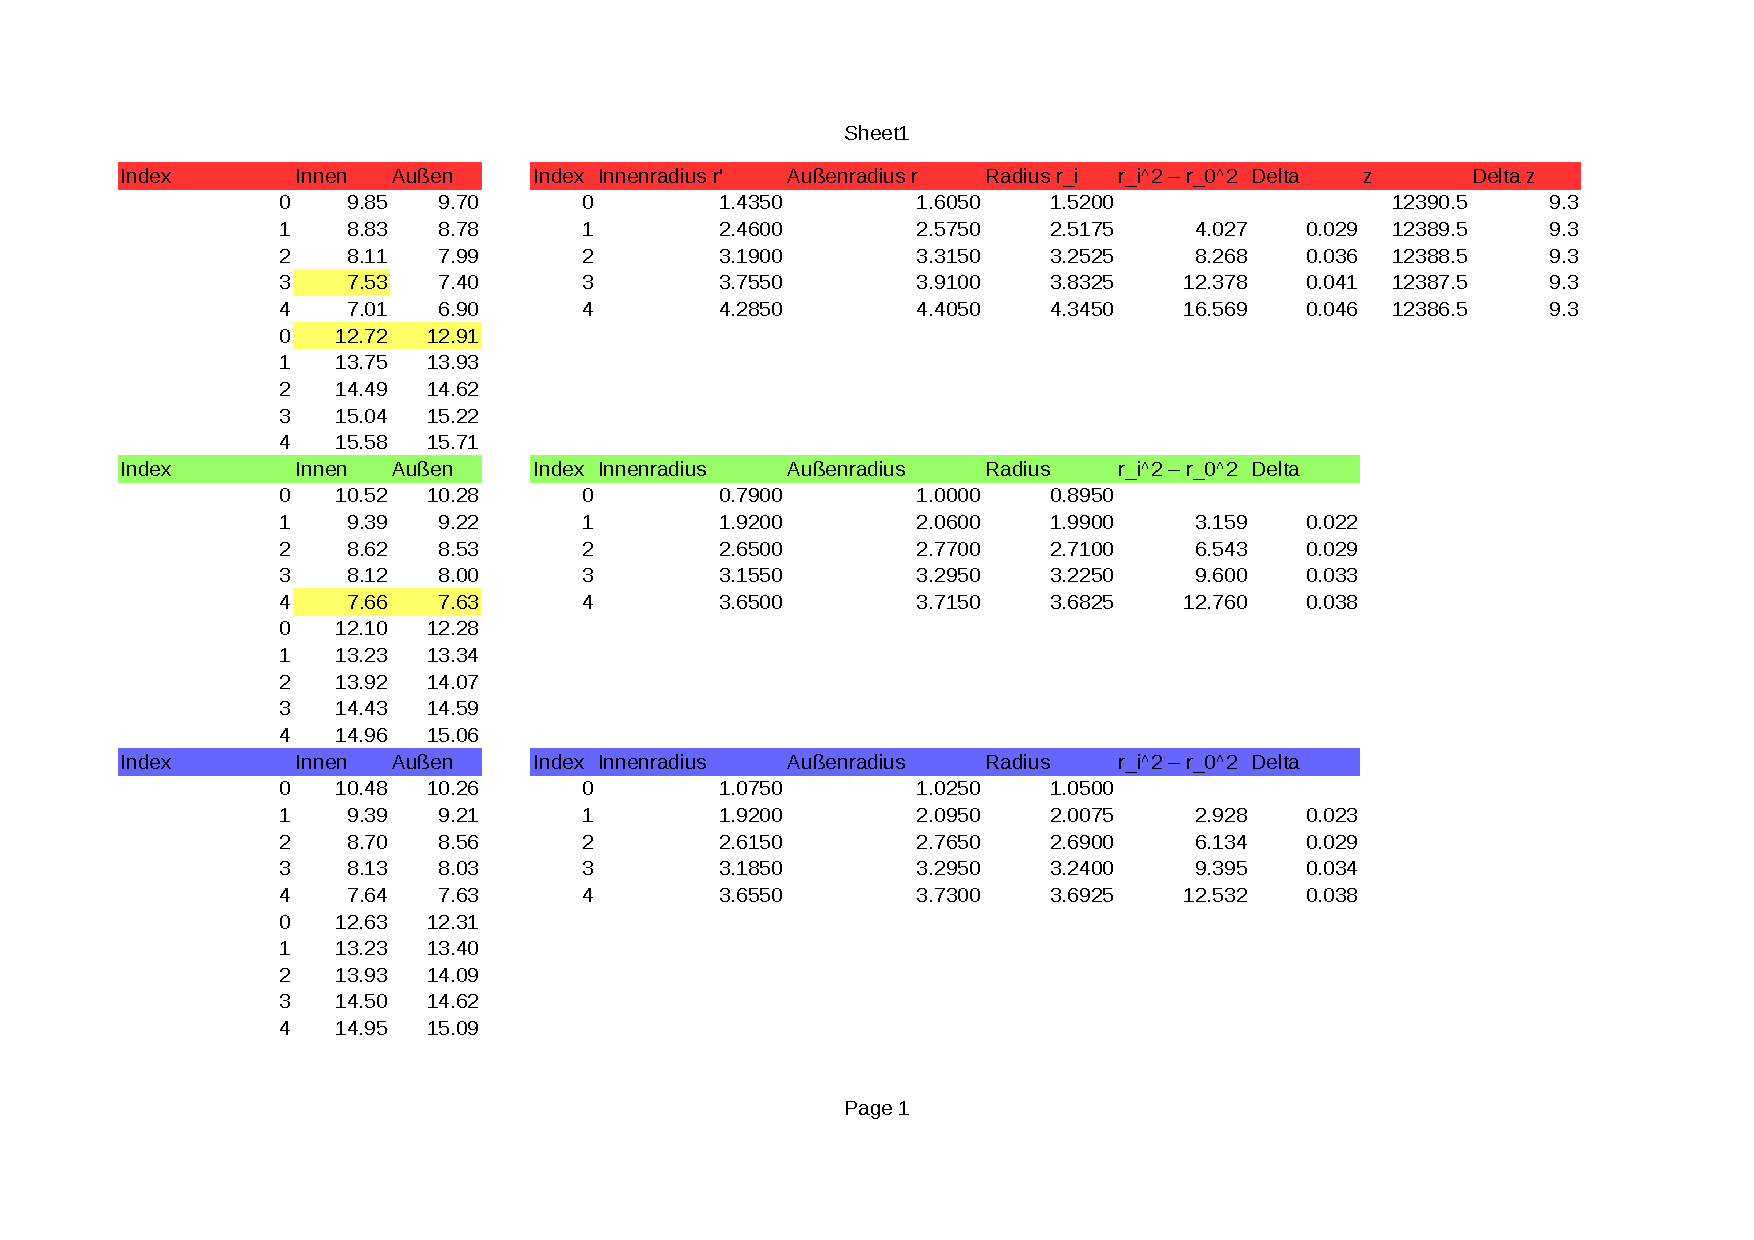
\includepdf{FAP-calc.pdf}
\end{document}